%Copyright 2019 Christopher M. Jermaine (cmj4@rice.edu) and Risa B. Myers (rbm2@rice.edu)
%
%Licensed under the Apache License, Version 2.0 (the "License");
%you may not use this file except in compliance with the License.
%You may obtain a copy of the License at
%
%    https://www.apache.org/licenses/LICENSE-2.0
%
%Unless required by applicable law or agreed to in writing, software
%distributed under the License is distributed on an "AS IS" BASIS,
%WITHOUT WARRANTIES OR CONDITIONS OF ANY KIND, either express or implied.
%See the License for the specific language governing permissions and
%limitations under the License.
\documentclass[aspectratio=169]{beamer}

%===============================================================%
\mode<presentation> 
{
\usetheme[noshadow, minimal,numbers,riceb,nonav]{Rice}
\usefonttheme[onlymath]{serif}
\setbeamercovered{transparent}
}
\useinnertheme{rectangles}

\usepackage[english]{babel}

\usepackage{mathptmx}
\usepackage{helvet}
\usepackage{courier}
\usepackage[T1]{fontenc}
\usepackage{trajan}
\usepackage{textcomp}
\usepackage{multirow}
\usepackage{xcolor,colortbl}

\usepackage{listings}

\newenvironment{noindentitemize}
{ \begin{itemize}
 \setlength{\itemsep}{1.5ex}
  \setlength{\parsep}{0pt}   
  \setlength{\parskip}{0pt}
 \addtolength{\leftskip}{-2em}
 }
{ \end{itemize} }

\newenvironment{noindentitemize2}
{ \begin{itemize}
  \setlength{\itemsep}{0ex}
  \setlength{\parskip}{0pt}
  \setlength{\parsep}{0pt}   
  \addtolength{\leftskip}{-2em}  }
{ \end{itemize} }




\setbeamerfont{block body}{size=\tiny}

%===============================================================%

\title[]
{Tools \& Models for Data Science}

\subtitle
{Relational Calculus}

\author[]{Chris Jermaine \& Risa Myers}
\institute
{
  Rice University
}

\date[]{}

\subject{Beamer}


\begin{document}


\begin{frame}
 \titlepage
\end{frame}

\begin{frame}{Relational Calculus}

\begin{itemize}
\item Nothing more than a First Order Logic predicate...
\item Embedded within a set constructor
\end{itemize}
\end{frame}
%***********************************************************
\begin{frame}{Writing RC Expressions}

Start with the easy parts

Recall the syntax $\{ t | P(t) \}$

\begin{enumerate}
\item Start with $\{ \}$
\item and the ``such that'' bar, |
\item  Then add in what you are looking for to the left of the |. 
   This is a description of the tuples you want back
\item  Then work on the right hand side
\item  Provide a predicate that evaluates to True over all the variables that appear on the left
\item If the predicate evaluates to True, that tuple will be included in the result set
\end{enumerate}
\end{frame}


%***********************************************************
\begin{frame}{Some Notations and Conventions}
Be sure to only include tuples that are in our relation(s)

Denoted as
\begin{itemize}
\item FREQUENTS(f)\\
 
 OR \\

\item FREQ(f)\\

OR\\

\item f $\in$ FREQ
\end{itemize}


\end{frame}

%***********************************************************
\begin{frame}{Example: Cold Brew Drinkers}

LIKES (DRINKER, COFFEE)

FREQUENTS (DRINKER, CAFE)

SERVES (CAFE, COFFEE)

\begin{itemize}
\item[?] Query: Who goes to a cafe serving Cold Brew?
\end{itemize}
\end{frame}

%***********************************************************
\begin{frame}{Example: Cold Brew  Drinkers}

LIKES (DRINKER, COFFEE)

FREQUENTS (DRINKER, CAFE)

SERVES (CAFE, COFFEE)

\begin{itemize}
\item Query: Who goes to a cafe serving Cold Brew?

\vspace{10 pt}
$\{f.\textrm{DRINKER } | \textrm{ FREQUENTS}(f) \wedge\ \exists(s)(\textrm{SERVES}(s)$

$\wedge\ s.\textrm{COFFEE} = \textrm{\textquotesingle{Cold} Brew\textquotesingle}
	\wedge\ s.\textrm{CAFE} = f.\textrm{CAFE})\}$
\end{itemize}
\end{frame}

%***********************************************************
\begin{frame}{Example: Cold Brew  Haters}

LIKES (DRINKER, COFFEE)

FREQUENTS (DRINKER, CAFE)

SERVES (CAFE, COFFEE)

\begin{itemize}
\item[?] Query: Who has not gone to a cafe serving Cold Brew?
\end{itemize}
\end{frame}

%***********************************************************
\begin{frame}{Example:Cold Brew  Haters, Common Approach}

LIKES (DRINKER, COFFEE)

FREQUENTS (DRINKER, CAFE)

SERVES (CAFE, COFFEE)

\begin{itemize}
\item Query: Who has not gone to a cafe serving Cold Brew?

\vspace{10 pt}
$\{f.\textrm{DRINKER } | \textrm{ FREQUENTS}(f) \wedge \neg \exists(s)(\textrm{SERVES}(s)$

$\wedge\ s.\textrm{COFFEE} = \textrm{\textquotesingle{Cold} Brew\textquotesingle}
	\wedge\ s.\textrm{CAFE} = f.\textrm{CAFE})\}$
\end{itemize}
\end{frame}

%***********************************************************
\begin{frame}{Example: Cold Brew  Haters, Common Approach}

LIKES (DRINKER, COFFEE)

FREQUENTS (DRINKER, CAFE)

SERVES (CAFE, COFFEE)

\begin{itemize}
\item Query: Who has not gone to a cafe serving Cold Brew?

\vspace{10 pt}
$\{f.\textrm{DRINKER} | \textrm{ FREQUENTS}(f) \wedge \neg \exists(s)(\textrm{SERVES}(s)$

$\wedge\ s.\textrm{COFFEE} = \textrm{\textquotesingle{Cold} Brew\textquotesingle}
	\wedge\ s.\textrm{CAFE} = f.\textrm{CAFE})\}$
\end{itemize}

\vspace{10 pt}
\begin{itemize}
\item Wrong!  This gives us ``Who has gone to a cafe that does not serve Cold Brew''

\item In parenthesis we have cafes that serve `Cold Brew' that someone has visited.

\item Negating it, and checking for existence, gives us cafes that someone has visited that do NOT serve Cold Brew.
\end{itemize}


\end{frame}

%***********************************************************
\begin{frame}{Walk--through Data}

%\hspace{-2em}Option A: Who has  gone to a cafe that does not serve `Cold Brew'?\\
%$\{f.\textrm{DRINKER } | \textrm{ FREQUENTS}(f) \wedge \neg \exists(s)(\textrm{SERVES}(s)$
%
%\hspace{2em}$\wedge\ s.\textrm{COFFEE} = \textrm{\textquotesingle{Cold} Brew\textquotesingle}
%	\wedge\ s.\textrm{CAFE} = f.\textrm{CAFE})\}$\\
%\vspace{2em}
%\hspace{-2em}Option B: Who has not gone to a cafe serving `Cold Brew'?\\
%$\{f.\textrm{DRINKER } | \textrm{FREQUENTS}(f) \wedge\ \neg \exists(f_2,s)(FREQ(f_2) $\\
%\hspace{2em}$\wedge\ SERVES(s) \wedge f_2.CAFE = s.CAFE $\\
%\hspace{2em}$\wedge\ s.COFFEE =  \textrm{\textquotesingle{Cold Brew}\textquotesingle} \wedge\ f.DRINKER = f_2.DRINKER) \}$
%
\begin{columns}[t]
\begin{column}{0.5\textwidth}
FREQUENTS\\
\begin{tabular}{|l|c|c| }  \hline
\textrm{DRINKER} & \textrm{CAFE}\\ \hline
Chris & A \\ \hline
Chris & B\\ \hline
Chris & C  \\ \hline
Risa & A\\ \hline
Risa & B \\ \hline
\end{tabular}
\end{column}
\begin{column}{0.5\textwidth}
SERVES\\
\begin{tabular}{|l|c|c| }  \hline
\textrm{CAFE} & \textrm{COFFEE}\\ \hline
A & Drip\\ \hline
A & Cold Brew \\ \hline
A &  Espresso \\ \hline
B & Drip  \\ \hline
C & Espresso \\ \hline
\end{tabular}
\end{column}
\end{columns}
\end{frame}
%***********************************************************
\begin{frame}{Common Approach}
\hspace{-2em}Who has gone to a cafe that does not serve `Cold Brew'?\\
$\{f.\textrm{DRINKER } | \textrm{ FREQUENTS}(f) \wedge \neg \exists(s)(\textrm{SERVES}(s)$

\hspace{2em}$\wedge\ s.\textrm{COFFEE} = \textrm{\textquotesingle{Cold} Brew\textquotesingle}
	\wedge\ s.\textrm{CAFE} = f.\textrm{CAFE})\}$\\
\hspace{-2em} For convenience, let's say:
 
\hspace{-2em} hasCB $ = \textrm{SERVES}(s) \wedge\ s.\textrm{CAFE} = f.\textrm{CAFE}\wedge\ s.\textrm{COFFEE} = \textrm{\textquotesingle{Cold} Brew\textquotesingle}$
\end{frame}

%***********************************************************
\begin{frame}{Common Approach Steps}


\begin{enumerate}
\item Start with the FREQUENTS table
\item Then look at matches in the SERVES table, where s.CAFE = f.CAFE
\item Evaluate the predicate
\item Is it TRUE?
\begin{itemize}
\item If Yes, then include f.DRINKER in the result set
\end{itemize}
\item When f.CAFE = `B', Risa gets included in the result set.

\hspace{-1em}
\begin{tabular}{|l|l|l|p{2cm}||l|l||l|}  \hline
\textrm{DRINKER} & \textrm{CAFE} &  \textrm{CAFE} &  \textrm{COFFEE} &\textrm{hasCB} &  $\neg$\textrm{hasCB} & \textrm{Result Set}\\ \hline
 Risa & B  & B & Drip & F& T & \{Risa\}\\ \hline 
 \end{tabular}

\item When f.CAFE = `A', Risa does NOT get add to the  result set

\hspace{-1em}
\begin{tabular}{|l|l|l|p{2cm}||l|l||l|}  \hline
\textrm{DRINKER} & \textrm{CAFE} &  \textrm{CAFE} &  \textrm{COFFEE} &\textrm{hasCB} &  $\neg$\textrm{hasCB} & \textrm{Result Set}\\ \hline
&  \multirow{3}{*}A & A & Drip &  \multirow{3}{*}T  &  \multirow{3}{*}F &  \multirow{3}{*}{ \{ \}} \\  \cline{3-4}
 Risa& & A& Cold Brew &   & & \\  \cline{3-4}
 & & A & Espresso &  & & \\ \hline
\end{tabular}

\end{enumerate}


\end{frame}

%***********************************************************
\begin{frame}{Common Approach Final Result}
\begin{itemize}
\item To get the final result set, we union together all the results from the final column

\hspace{-1em}
\begin{tabular}{|l|l|l|p{2cm}||l|l||l|}  \hline \hline
\color{white}\textrm{DRINKER} & \color{white}\textrm{CAFE} & \color{white} \textrm{CAFE} &  \color{white}\textrm{COFFEE} &\color{white}\textrm{hasCB} & \color{white} $\neg$\textrm{hasCB} &\color{white} \textrm{Result Set}\\ 

& & & & & & \{ Risa \} \\ \hline
 \end{tabular}

\item The final result set is \{ Risa \} $\cup$ \{ \}  = \{ Risa \}
\item However, Risa shouldn't be in the result set, because she frequents Cafe A, which serves Cold Brew 
\item Issue: We want to look at ALL of the coffees served at ALL of the cafes Risa frequents all at one time
\end{itemize}


\end{frame}



%***********************************************************
\begin{frame}{Correct Approach}

Who has not gone to a cafe serving `Cold Brew'?\\
\begin{itemize}
\item To answer this question, we need to introduce a second variable:

$\{f_1.\textrm{DRINKER } | \textrm{FREQUENTS}(f_1) \wedge\ \neg \exists(f_2,s)(FREQ(f_2) $

\hspace{2em} $\wedge\ SERVES(s) \wedge f_2.CAFE = s.CAFE $

\hspace{2em} $\wedge\ s.COFFEE =  \textrm{\textquotesingle{Cold Brew}\textquotesingle} \wedge\ f_1.DRINKER = f_2.DRINKER) \}$


\item Again, for convenience, let's say:
 
hasCB $ =(FREQ(f_2) $

\hspace{2em} $\wedge\ SERVES(s) \wedge f_2.CAFE = s.CAFE $

\hspace{2em} $\wedge\ s.COFFEE =  \textrm{\textquotesingle{Cold Brew}\textquotesingle} \wedge\ f_1.DRINKER = f_2.DRINKER) $
\end{itemize}


\end{frame}

%***********************************************************
\begin{frame}{Correct Approach}
In this case, by having the second variable, we are able to look at all the data for every place Risa frequents as a whole.

\begin{itemize}
\item Here, we have another variable, $f_2$
\item We consider each drinker in turn from the FREQUENTS relation. Basically, we are using this table as our master list of drinkers, and are ignoring the CAFE attribute.

Again, look just at Risa.

%
%\begin{tabular}{|l|}  \hline
%\textrm{DRINKER} \\ \hline
%Risa \\ \hline
%\end{tabular}


\item Now, look at all the combinations of FREQUENTS and SERVES where the CAFE matches and the drinker is $f_1$.DRINKER 
\scriptsize{
\begin{tabular}{|l|l|l|l|p{2cm}||l|l||l|}  \hline 
\textrm{$f_1$.DRINKER} &\textrm{$f_2$.DRINKER} & \textrm{CAFE} &  \textrm{CAFE} &  \textrm{COFFEE} &\textrm{hasCB} &  $\neg$\textrm{hasCB} & \textrm{Result Set}\\ \hline
 & Risa & A & A & Cold Brew & \multirow{3}{*}T & \multirow{3}{*}F &  \multirow{3}{*}{\{ \}}\\ \cline{2-5}
Risa &Risa & A  & A & Drip & & & \\ \cline{2-5}
 & Risa & A  & A & Espresso & &  &\\ \cline{2-5}
 & Risa & B  & B & Drip & & & \\ \hline
\end{tabular}
}
\item If there is any tuple where the Coffee is `Cold Brew', we exclude the drinker


\item Now, in this case, one of the cafes that Risa frequents does serve Cold Brew, so Risa is not added to the result set
\end{itemize}

\end{frame}

%***********************************************************
%\begin{frame}{Example: Not Bad Coffee People}
%
%LIKES (DRINKER, COFFEE)
%
%FREQUENTS (DRINKER, CAFE)
%
%SERVES (CAFE, COFFEE)
%
%\begin{itemize}
%\item Query: Who has not gone to a cafe serving Cold Brew?
%
%\vspace{10 pt}
%$\{f.\textrm{DRINKER } | \textrm{ FREQUENTS}(f) \wedge\
%	\forall(f_2)(\textrm{FREQUENTS}(f_2)$
%
%$\wedge\ f.\textrm{DRINKER} = f_2.\textrm{DRINKER} \rightarrow
% \neg \exists(s)(\textrm{SERVES}(s)$
%
%$\wedge\ s.\textrm{COFFEE} = \textrm{\textquotesingle{Cold Brew}\textquotesingle}
%	\wedge\ s.\textrm{CAFE} = f_2.\textrm{CAFE}))\}$
%\end{itemize}
%
%\begin{itemize}
%\item[?] Why do we need both $f$ and $f_2$ here?
%\item[?] Note: we invariably have a ``$\rightarrow$'' within a $\forall$ quantifier.  Why?
%\end{itemize}
%\vspace{10 pt}
%\end{frame}
%
%%***********************************************************
%\begin{frame}{Example: Not Bad Coffee People}
%\begin{itemize}
%\item Why do we need both $f$ and $f_2$ here?
%\begin{itemize}
%\item $\forall$ goes to the universe, looking at all possible values
%\item The universe can contain things we don't care about
%\item So, we want to ensure that $f_2$ is in DRINKER
%\item And refers to the correct drinker
%%\item For every tuple $f_2$, if $f_2$ refers to the same drinker as $f$, then $f_2$ had better not show that the person is going to a bad cafe
%\end{itemize}
%\item Note: we invariably have a ``$\rightarrow$'' within a $\forall$ quantifier.  Why?
%\begin{itemize}
%\item $\rightarrow$ is a logical IF--THEN statement
%\end{itemize}
%\end{itemize}
%
%\end{frame}
%
%***********************************************************
\begin{frame}{Example: People Who Like to Drink Coffee}

LIKES (DRINKER, COFFEE)

FREQUENTS (DRINKER, CAFE)

SERVES (CAFE, COFFEE)

\begin{itemize}
\item[?] Query: Who goes to a cafe that serves a coffee they like?
\end{itemize}
\end{frame}

%***********************************************************
\begin{frame}{Example: People Who Like to Drink Coffee}

LIKES (DRINKER, COFFEE)

FREQUENTS (DRINKER, CAFE)

SERVES (CAFE, COFFEE)

\begin{noindentitemize}
\item Query: Who goes to a cafe that serves a coffee they like?

\vspace{10 pt}
$\{f.\textrm{DRINKER } | \textrm{ FREQUENTS}(f) \wedge \exists(s, l)(\textrm{SERVES}(s) \wedge \textrm{LIKES}(l)$

\hspace{2em} $\wedge\ s.\textrm{COFFEE} = l.\textrm{COFFEE}$

\hspace{2em} $\wedge\ s.\textrm{CAFE} = f.\textrm{CAFE}$

\hspace{2em} $\wedge\ l.\textrm{DRINKER} = f.\textrm{DRINKER}) \}$

\item[?] We didn't refer to any table more than once. Why not?
\end{noindentitemize}
\end{frame}

%***********************************************************
\begin{frame}{Example: People Who Like to Drink Coffee}

LIKES (DRINKER, COFFEE)

FREQUENTS (DRINKER, CAFE)

SERVES (CAFE, COFFEE)

\begin{noindentitemize}
\item Query: Who goes to a cafe that serves a coffee they like?

\vspace{10 pt}
$\{f.\textrm{DRINKER } | \textrm{ FREQUENTS}(f) \wedge \exists(s, l)(\textrm{SERVES}(s) \wedge \textrm{LIKES}(l)$

\hspace{2em} $\wedge\ s.\textrm{COFFEE} = l.\textrm{COFFEE}$

\hspace{2em} $\wedge\ s.\textrm{CAFE} = f.\textrm{CAFE}$

\hspace{2em} $\wedge\ l.\textrm{DRINKER} = f.\textrm{DRINKER}) \}$

\item We didn't refer to any table more than once. Why not?
\item It wasn't needed since we didn't have any `Always' or `Never' predicates
\item We were looking for `Any'
\end{noindentitemize}
\end{frame}


%***********************************************************
%\begin{frame}{Example: Super Cool Cafes}
%
%LIKES (DRINKER, COFFEE)
%
%FREQUENTS (DRINKER, CAFE)
%
%SERVES (CAFE, COFFEE)
%
%\begin{noindentitemize}
%\item[?] Query: Which cafes serve all of the coffees that Risa likes?
%\end{noindentitemize}
%\end{frame}
%
%%***********************************************************
%\begin{frame}{Example: Super Cool Cafes}
%
%LIKES (DRINKER, COFFEE)
%
%FREQUENTS (DRINKER, CAFE)
%
%SERVES (CAFE, COFFEE)
%
%\begin{noindentitemize}
%\item Query: Which cafes serve all of the coffees that Risa likes?
%
%\vspace{10 pt}
%$\{s.\textrm{CAFE } | \textrm{ SERVES}(s) \wedge \forall(l)(\textrm{if } l \textrm{ is from LIKES and}$
%
%\hspace{2em} $\textrm{corresponds to \textquotesingle{Risa}\textquotesingle, then the cafe serves it})\}$
%\end{noindentitemize}
%\end{frame}
%
%%***********************************************************
%\begin{frame}{Example: Super Cool Cafes}
%
%LIKES (DRINKER, COFFEE)
%
%FREQUENTS (DRINKER, CAFE)
%
%SERVES (CAFE, COFFEE)
%
%\begin{noindentitemize}
%\item Query: Which cafes serve all of the coffees that Risa likes?
%
%\vspace{10 pt}
%$\{s.\textrm{CAFE } | \textrm{ SERVES}(s) \wedge \forall(l)(\textrm{LIKES}(l)\wedge\ l.\textrm{DRINKER} = \textrm{\textquotesingle{Risa}\textquotesingle}$
%
%\hspace{2em} $\rightarrow \exists(s_2)(\textrm{SERVES}(s_2)$
%
%\hspace{4em} $ \wedge\ s_2.\textrm{CAFE} = s.\textrm{CAFE} \wedge s_2.\textrm{COFFEE} = l.\textrm{COFFEE}))\}$
%\end{noindentitemize}
%\end{frame}
%
%***********************************************************
\begin{frame}{Example: People Who Avoid Bad Cafes} % The coffee snob example

LIKES (DRINKER, COFFEE)

FREQUENTS (DRINKER, CAFE)

SERVES (CAFE, COFFEE)

\begin{noindentitemize}
\item[?] Query: Which people only go to cafes that serve a coffee they like?
\end{noindentitemize}
\end{frame}
%***********************************************************
\begin{frame}{Example: People Who Avoid Bad Cafes}

LIKES (DRINKER, COFFEE)

FREQUENTS (DRINKER, CAFE)

SERVES (CAFE, COFFEE)

\begin{noindentitemize}
\item[?] Query: Which people only go to cafes that serve a coffee they like?
\end{noindentitemize}
\end{frame}


%***********************************************************
\begin{frame}{Example: People Who Avoid Bad Cafes}

LIKES (DRINKER, COFFEE)

FREQUENTS (DRINKER, CAFE)

SERVES (CAFE, COFFEE)

\begin{noindentitemize}
\item Query: Which people only go to cafes that serve a coffee they like?

\vspace{10 pt}
$\{f.\textrm{DRINKER } | \textrm{ FREQUENTS}(f) \wedge \forall(f_2)(\textrm{if } f_2 \textrm{ tells us a cafe that }$

\hspace{2em}$f.\textrm{DRINKER goes to then that cafe needs to serve a coffee that}$
 
\hspace{2em}$f.\textrm{DRINKER likes})\}$
\end{noindentitemize}
\end{frame}

%***********************************************************
\begin{frame}{Example: People Who Avoid Bad Cafes}

LIKES (DRINKER, COFFEE)

FREQUENTS (DRINKER, CAFE)

SERVES (CAFE, COFFEE)

\begin{noindentitemize}
\item Query: Which people only go to cafes that serve a coffee they like?

\vspace{10 pt}
$\{f.\textrm{DRINKER } | \textrm{ FREQUENTS}(f) \wedge \forall(f_2)(\textrm{FREQUENTS}(f_2)$

\hspace{2em}$\wedge\ f.\textrm{DRINKER} = f_2.\textrm{DRINKER} \rightarrow \exists(s, l)(\textrm{SERVES}(s)$

\hspace{2em}$ \wedge\ \textrm{LIKES}(l) \wedge\ s.\textrm{CAFE} = f_2.\textrm{CAFE} \wedge\ l.\textrm{COFFEE} = s.\textrm{COFFEE}$

\hspace{2em}$\wedge\	l.\textrm{DRINKER} = f_2.\textrm{DRINKER}))\}$

\end{noindentitemize}
\end{frame}

%***********************************************************
\begin{frame}{Implication}

$\{f.\textrm{DRINKER } | \textrm{ FREQUENTS}(f) \wedge \forall(f_2)(\textrm{FREQUENTS}(f_2)$

\hspace{2em}$\wedge\ f.\textrm{DRINKER} = f_2.\textrm{DRINKER} \rightarrow \exists(s, l)(\textrm{SERVES}(s)$

\hspace{2em}$ \wedge\ \textrm{LIKES}(l) \wedge\ s.\textrm{CAFE} = f_2.\textrm{CAFE} \wedge\ l.\textrm{COFFEE} = s.\textrm{COFFEE}$

\hspace{2em}$\wedge\	l.\textrm{DRINKER} = f_2.\textrm{DRINKER}))\}$

\begin{itemize}
\item[?] Note: we invariably have a ``$\rightarrow$'' within a $\forall$ quantifier.  Why?
\end{itemize}
\end{frame}
%***********************************************************
\begin{frame}{Implication}

$\{f.\textrm{DRINKER } | \textrm{ FREQUENTS}(f) \wedge \forall(f_2)(\textrm{FREQUENTS}(f_2)$

\hspace{2em}$\wedge\ f.\textrm{DRINKER} = f_2.\textrm{DRINKER} \rightarrow \exists(s, l)(\textrm{SERVES}(s)$

\hspace{2em}$ \wedge\ \textrm{LIKES}(l) \wedge\ s.\textrm{CAFE} = f_2.\textrm{CAFE} \wedge\ l.\textrm{COFFEE} = s.\textrm{COFFEE}$

\hspace{2em}$\wedge\	l.\textrm{DRINKER} = f_2.\textrm{DRINKER}))\}$

\begin{itemize}
\item Note: we invariably have a ``$\rightarrow$'' within a $\forall$ quantifier.  Why?
\begin{itemize}
\item $\rightarrow$ is a logical IF--THEN statement
\end{itemize}
\end{itemize}
\end{frame}
%***********************************************************
\begin{frame}{Implication}

$\{f.\textrm{DRINKER } | \textrm{ FREQUENTS}(f) \wedge \forall(f_2)(\textrm{FREQUENTS}(f_2)$

\hspace{2em}$\wedge\ f.\textrm{DRINKER} = f_2.\textrm{DRINKER} \rightarrow \exists(s, l)(\textrm{SERVES}(s)$

\hspace{2em}$ \wedge\ \textrm{LIKES}(l) \wedge\ s.\textrm{CAFE} = f_2.\textrm{CAFE} \wedge\ l.\textrm{COFFEE} = s.\textrm{COFFEE}$

\hspace{2em}$\wedge\	l.\textrm{DRINKER} = f_2.\textrm{DRINKER}))\}$

\vspace{-2em}

 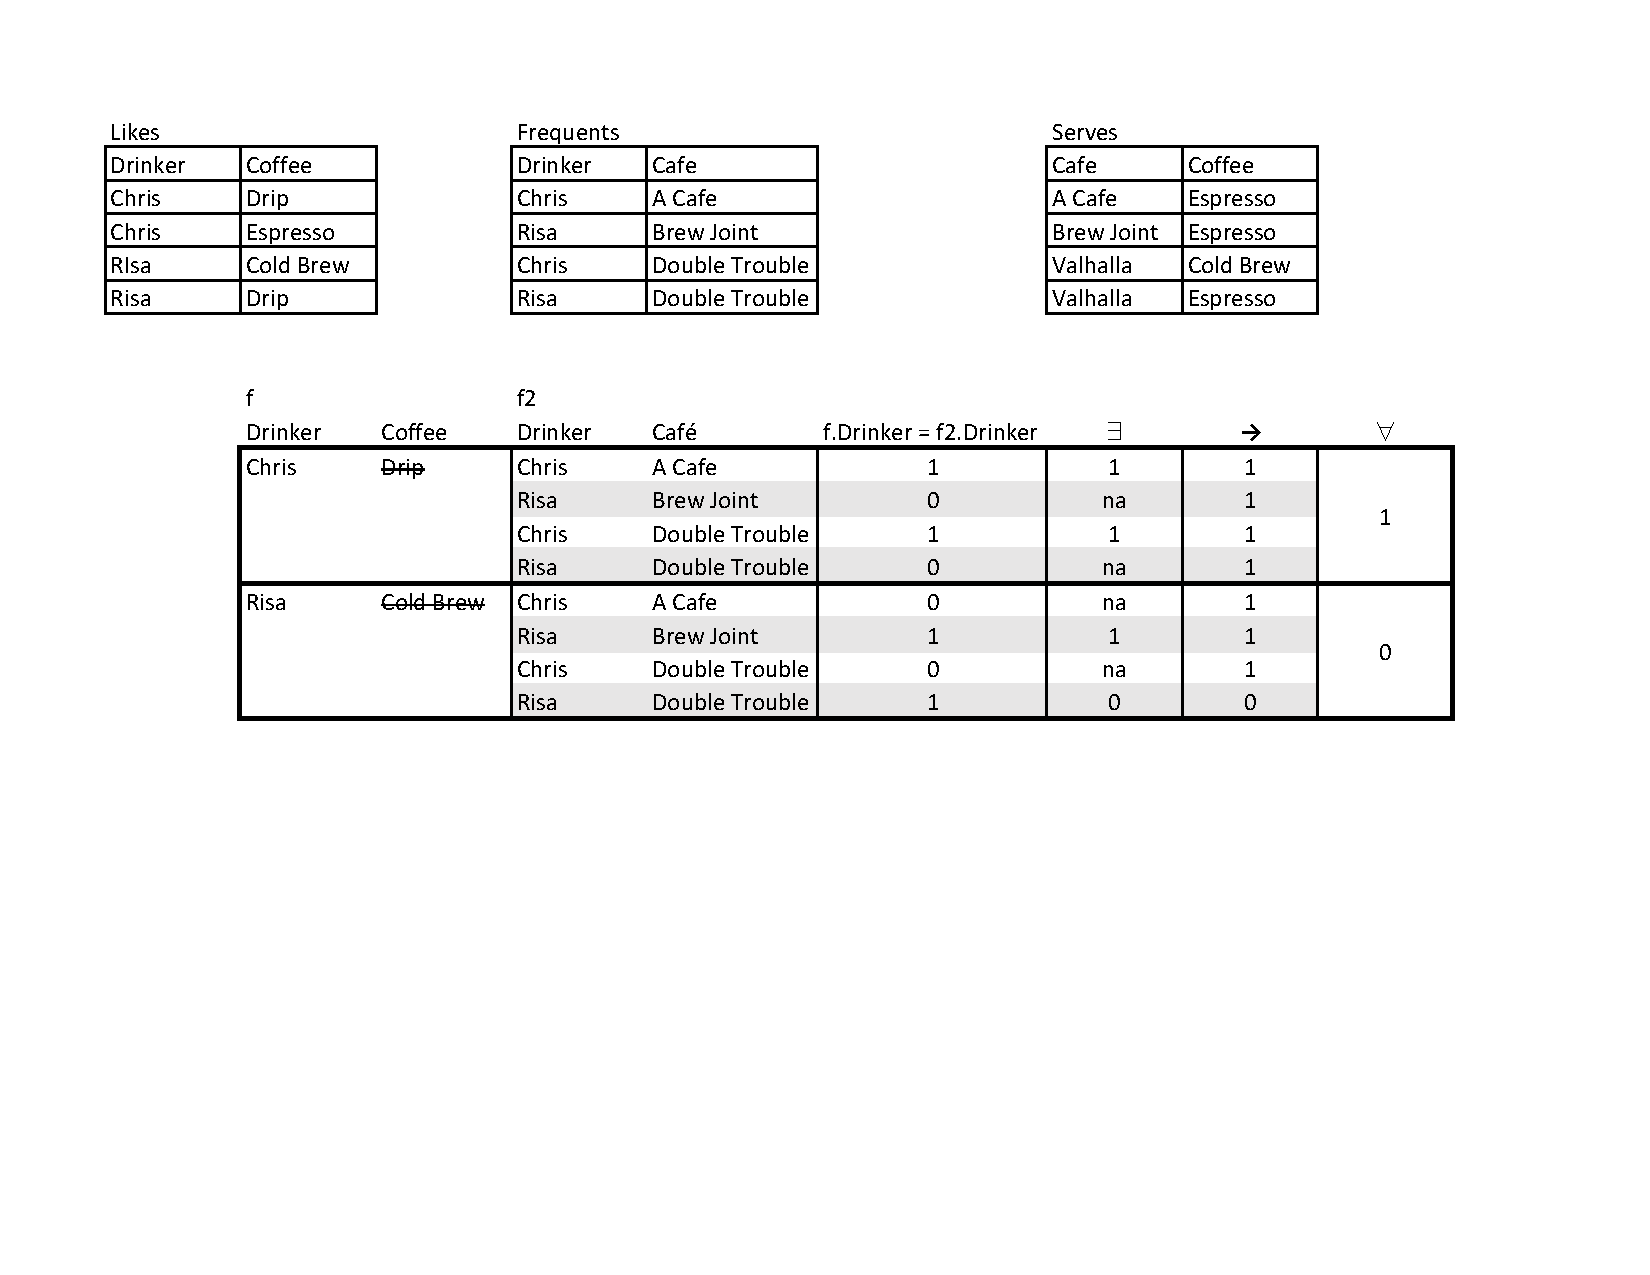
\includegraphics[width=1\textwidth]{./lectRCRA/drinkerFrequentsServes.pdf}
\end{frame}


%***********************************************************

\begin{frame}{Wrap up}
\begin{enumerate}
\item What is Relational Calculus?
% variant of first order logic
% foundation of SQL
\item Why does it matter?
% gets us thinking declaratively
% foundation of SQL
\end{enumerate}

\begin{itemize}
	\item[?] How can we use what we learned today?
	\vspace{2em}
	\item[?] What do we know now that we didn't know before?
\end{itemize}


\end{frame}

\end{document}
